
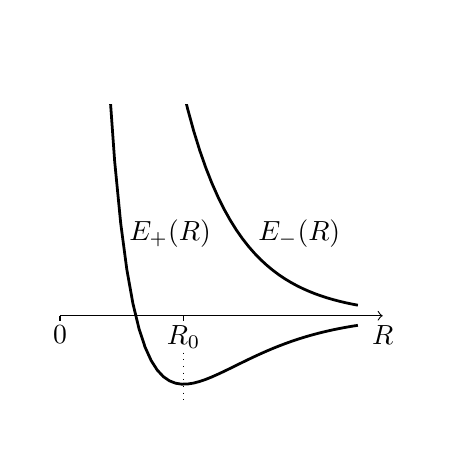
\begin{tikzpicture}[
declare function={ 
	K(\r) = -1 * exp(-1 * \r) * (1 + \r);
	S(\r) = exp(-1 * \r) * (1 + \r + \r ^2 / 3);
	J(\r) = exp(-2 * \r) * (1 + 1/\r) - 1 / \r;	
	austausch(\r) = - S(\r) / 2 + K(\r) + S(\r) / \r;
	coulomb(\r) = -1/2 + J(\r) + 1/\r;
	up(\r) = (coulomb(\r) + austausch(\r)) / (1 + S(\r)) + 0.5;
	um(\r) = (coulomb(\r) - austausch(\r)) / (1 - S(\r)) + 0.5;
  },
]
\useasboundingbox (0,0) rectangle (5,5);
%\draw (0,0) rectangle (5,5);

\begin{axis}[no markers, samples=50,
          ymin=-1, ymax=2,
        axis y line=none,
           axis x line=none,
           width= 6.5cm]
           
\addplot [domain=0:6,  line width=1pt]    {10 * up(x) };
\addplot [domain=0:6,  line width=1pt]    {10 * um(x) };

  
\addplot[->] coordinates   {(0,0) (6.5, 0)};
\addplot[] coordinates   {(0,0) (0, -0.05)};
\addplot[] coordinates   {(2.49,0) (2.49, -0.05)};
\addplot[dotted] coordinates   {(2.49,-0.35) (2.49, -0.8)};


\node[anchor=north] at (axis cs: 6.5,0) {$R$};
\node[anchor=north] at (axis cs: 2.49,0) {$R_0$};
\node[anchor=north] at (axis cs: 0,0) {$0$};

\node[anchor=north west] at (axis cs: 3.8,1) {$E_-(R)$};
\node[anchor=north west] at (axis cs: 1.2,1) {$E_+(R)$};



%\node[anchor=north] at (axis cs: +1,0) {$\mathbf{r}_2$};
%
%\node[anchor= north east] at (axis cs: -1,1) {$|\phi_1|^2$};
%\node[anchor= west] at (axis cs: +1.3,-0.7) {$\frac{-1}{|\mathbf{r} - \mathbf{r}_2|}$};
%
%\node (s) [anchor= west] at (axis cs: +1,+0.5) {$\frac{|\phi_1|^2}{|\mathbf{r} - \mathbf{r}_2|}$} ;
%
%\node (k) at (axis cs: -1,+0.) {};

%\draw (s) -- (k) ;

%\node[anchor= south] at (axis cs: 0,0) {$\phi_1 \cdot \phi_2$};

%\node[anchor=west] at (axis cs: 1,1.4) {state $e$};
           
\end{axis}

\end{tikzpicture}

